\documentclass{article}
\usepackage[margin=1in]{geometry}
\usepackage{graphicx}
\usepackage{xcolor}
\usepackage{float}
\usepackage{amsmath}
\usepackage{cite}
\usepackage{hyperref}
\graphicspath{{..} {./images}}

\definecolor{navy-blue}{rgb}{0.22,0.38,0.71}

\renewcommand{\contentsname}{\vspace*{-2\baselineskip}}

\hypersetup{
	colorlinks,
	linkcolor=black,
	urlcolor=blue,
	citecolor=black
}
  		
\begin{document}
\begin{titlepage}
	\centering
	{\huge Lab 4 - Analog Modulation with SDR}\\[0.25 in]
	
\includegraphics[width=0.6\textwidth]{ua_logo.png}\\[0.25 in]
	{\large \textbf{ECE 531 - Software Defined Radio\\[0.25 in]
	March 17, 2025\\[0.25 in]}}
	{\large Owen Sowatzke, osowatzke@arizona.edu\\[0.05 in]
	Department of Electrical \& Computer Engineering\\[0.05 in]
	University of Arizona, Tucson, AZ 85721\\[0.5 in]}
	\hypersetup{linkcolor=navy-blue}
	\noindent\hrulefill
	\tableofcontents
	\noindent\hrulefill
\end{titlepage}

\setlength{\parindent}{0pt}

\section{Introduction}
%Introduction to the laboratory experiment, including a brief description of the objectives and goals.

\section{Procedure}
% Detailed explanation of the laboratory experiment, including the design, implementation, and testing of the system.

\begin{figure}[H]
	\centerline{\fbox{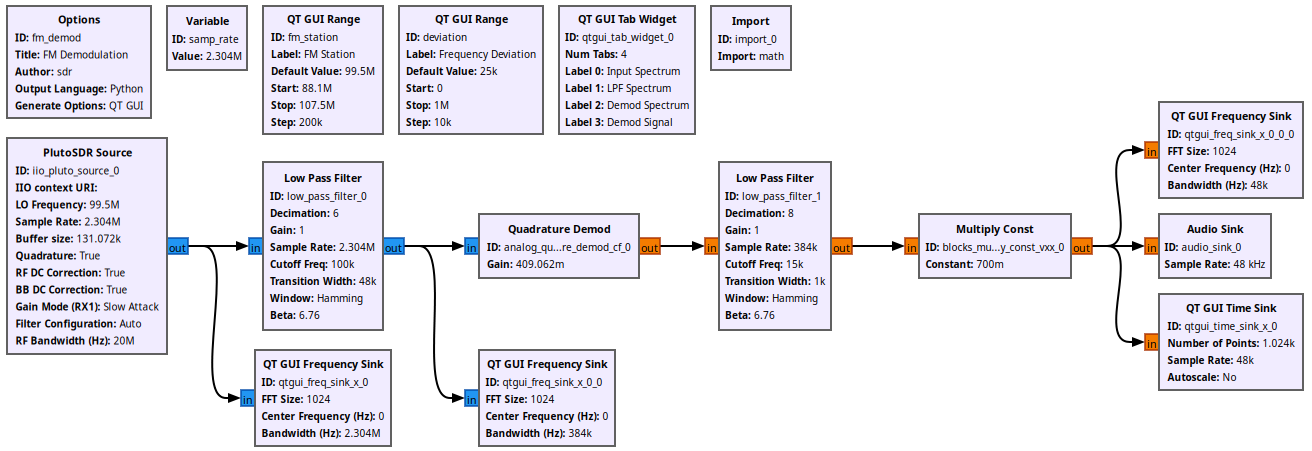
\includegraphics[width=0.7\textwidth]{fm_radio_flowchart.png}}}
	\caption{Flowchart for FM Demodulation}
	\label{fig::fm_radio_flowchart}
\end{figure}

\section{Results}
% Results and discussion of the laboratory experiment, including captured outputs, observations, and responses to laboratory questions.

At 99.5 FM:

\begin{figure}[H]
	\centerline{\fbox{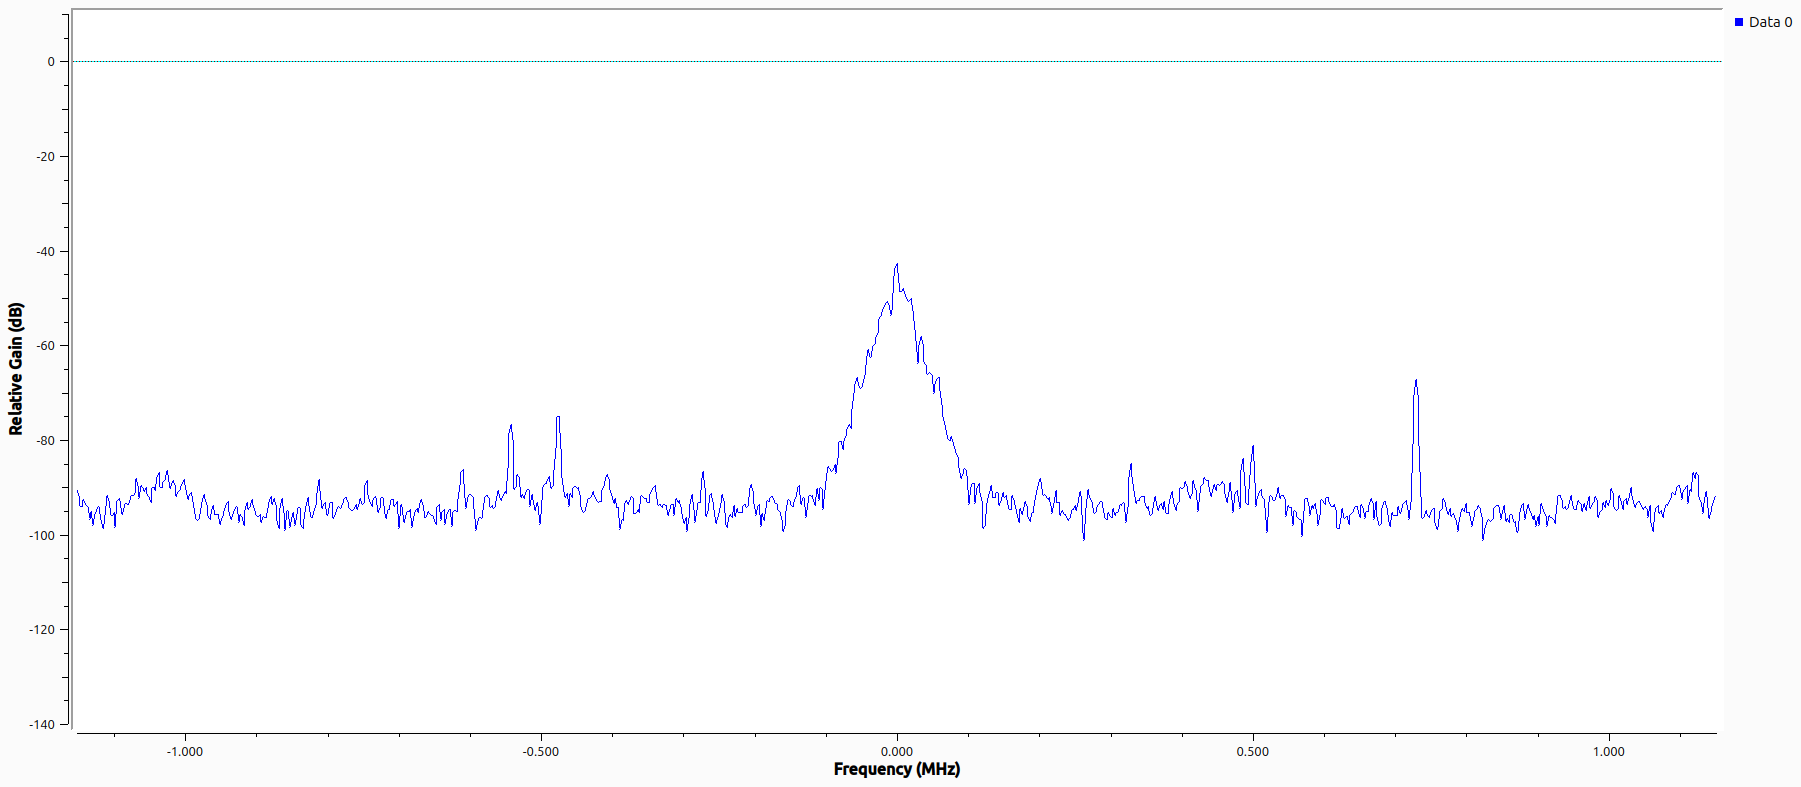
\includegraphics[width=0.7\textwidth]{spectrum_before_demodulation.png}}}
	\caption{FM Radio Spectrum Before Demodulation}
	\label{fig::spectrum_before_demodulation}
\end{figure}

\begin{figure}[H]
	\centerline{\fbox{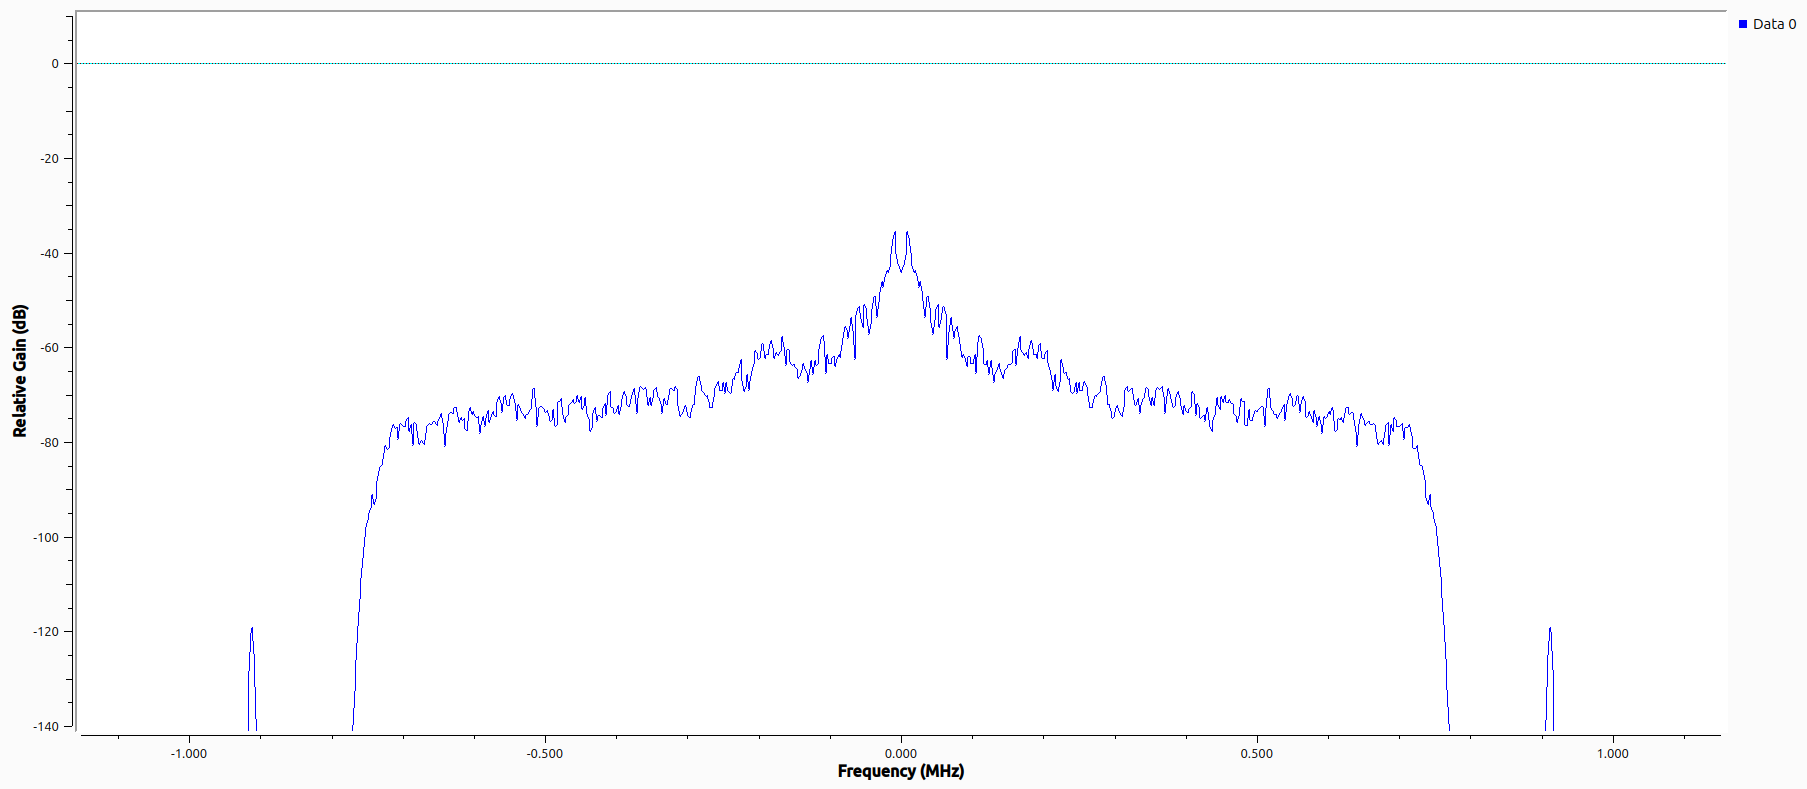
\includegraphics[width=0.7\textwidth]{spectrum_after_demodulation.png}}}
	\caption{FM Radio Spectrum After Demodulation}
	\label{fig::spectrum_after_demodulation}
\end{figure}

There are two decimation filters within the block diagram. One is before the FM demodulation block and limits the bandwidth of the signal to the width of the RF channel. The second filter is included with the FM demodulation block, and it limits the frequency of the audio output for the audio sink. The first filter provides a decimation rate of 6, and the second filter provides a decimation rate of 8. As a result, our sample rate falls from 2.304 MHz to 48 kHz, which is exactly the sample rate we need for the audio source.

A rational resampler block would be needed instead of decimating FIRs if the input sampling rate is not a multiple of the audio sink sampling rate. In Figure \ref{fig::fm_radio_flowchart}, the input sampling rate is a multiple of the audio sink sampling rate (i.e. $48\ \text{kHz} \times 48 = 2.304\ \text{MHz}$).

The resulting audio quality is not bad. However, the audio contains noise and occasional gaps due to the USB having trouble keeping up with the input data rates. All the noise at frequencies outside of the interval $[-f_s/2, +f_s/2) = [-1.652\ \text{MHz}, 1.652\ \text{MHz})$ will alias back into the baseband spectrum - degrading the SNR. To improve the SNR, we can decrease the RF bandwidth. FM radio channels have a bandwidth of 200 kHz, so we want a bandwidth larger than this and less than the sample rate of 2.304 MHz. The 100 MHz cutoff frequency for the low-pass filter (LPF) is sized to the bandwidth of the RF channel instead of the output rate of the LPF. Because the filter bandwidth is less than the rate of the decimated rate, we have no problems with the lower rate. Choose a lower rate also reduces the amount of noise going into the FM demodulator.

\section{Conclusion}
% Conclusions to the overall lab that discuss meaningful lessons learned and other takeaways from the assignment. (Important)

%\nocite{analog_devices_libiio_error}
%\bibliographystyle{IEEEtran}
%\bibliography{sources}{}
%\bibliographystyle{ieeetr}
	
\end{document}